\documentclass{notes}
\usepackage[margin=1in]{geometry}

\usepackage{svg}
\usepackage{graphicx}
\usepackage{boldline}
\usepackage{textcomp}
\usepackage{listings}
% \usepackage[,table]{xcolor}
\definecolor{red}{cmyk}{0, 1.00, 0.62,0}
\definecolor{blue}{cmyk}{1.00, .34, .0 .02 }    % blue
\definecolor{green}{cmyk}{0.7, 0, 1.0, 0.09 }   % greenish
\definecolor{yellow}{cmyk}{0, 0.16, 1.0, 0}     % yellow
\definecolor{gray}{cmyk}{0, 0, 0, 0.65}         % gray
\definecolor{purple}{cmyk}{.333, .867, 0, .059}
\colorlet{codebase}{yellow!30!}
\colorlet{codekeyword}{blue}
\colorlet{codecomment}{green}
\colorlet{codestring}{red}
\lstset{
  language=Python,
  backgroundcolor=\color{codebase},   %\color[RGB]{250, 245, 182},
  tabsize=4,
  basewidth=.5em,
  rulecolor=\color{yellow},           %\color{black},
  basicstyle=\normalsize\ttfamily,    % code text size
  upquote=true,
  columns=fixed,
  extendedchars=true,
  breaklines=true,
  prebreak = \raisebox{0ex}[0ex][0ex]{\ensuremath{\hookleftarrow}},
  frame=lrtb,
  xleftmargin=5pt,
  xrightmargin=5pt,
  framesep=4pt,
  framerule=2pt,
  showtabs=false,
  showspaces=false,
  showstringspaces=false,
  keywordstyle=\color{codekeyword},   %\color[RGB]{42, 161, 152},
  commentstyle=\color{codecomment},   %\color[RGB]{108, 153, 8},
  stringstyle=\color{codestring},     %\color[RGB]{189, 78, 98},
  title=\lstname,
  captionpos=b,
  abovecaptionskip=-5pt,
  belowcaptionskip=-5pt,
  moredelim=[is][\color{black}]{<<}{>>},
  moredelim=[is][\color{red}]{<r<}{>r>},
  moredelim=[is][\color{blue}]{<b<}{>b>},
  moredelim=[is][\color{green}]{<g<}{>g>},
  moredelim=[is][\color{purple}]{<p<}{>p>},
  morekeywords={assert, bytes, self, super, with, as, yield, True, False, None, NotImplemented, BaseException, Exception, AssertionError, AttributeError, ImportError, IndexError, KeyError, KeyboardInterrupt, MemoryError, NameError, NotImplementedError, OSError, OverflowError, RecursionError, RuntimeError, StopIteration, SyntaxError, IndentationError, TabError, StandardError, SystemError, SystemExit, TypeError, ValueError, ZeroDivisionError, IOError, Warning, RuntimeWarning, FileExistsError, FileNotFoundError,
    SELECT, FROM, AS, INNER, JOIN, LEFT, OUTER, CROSS, ON, WHERE, CASE, IF,
    MIN, MAX, SUM, AVG, COUNT, TEXT, REAL
  }
}

\usepackage{hyperref}
\hypersetup{
  colorlinks = true,
  urlcolor = blue,
  linkcolor = blue,
  citecolor = red
}
% \setlength{\jot}{8pt}

\setlength{\tabcolsep}{16pt} % sets padding between text and left/right border
\setlength{\arrayrulewidth}{0.7pt}
\renewcommand{\arraystretch}{1.2}


\author{Erik Hannesson}
\title{Predictive Hockey Analytics}
\date{February 2020}

\begin{document}
  \maketitle
  \begin{abstract}
    It's pretty straightforward, really.
    We used the National Hockey League's (NHL) API to steal whatever data we could get our grimyc hands on, and then:\\

    \begin{center}
      {\Large \textbf{Linear Algebra}.}\footnote{See Figure~\ref{fig:xkcd-ml} for a helpful infographic.}
    \end{center}
    \hfill\\
    And that's about all you need to know.
  \end{abstract}

  \section{Motivation and Overview}


  \section{Data}
    So I'm pretty sure we already explained this in the abstract, but I guess we'll vomit it back up here.\\

    The NHL API provides both historical data and live feed data for games currently in play.
    This allows for incredible diversity in approach and application.\\

    There are two main categories of data that can be analyzed: team data and player data.
    These can be approached independently, or simultaneously.\\

    Here is a rundown of the main features we use.\\

    % TODO: this needs to be aligned properly (and skater stats need to actually be correct...)
      {\rowcolors{3}{white}{gray!15}
      \begin{tabular}{ |c|c| }
        \multicolumn{2}{c}{\textbf{Team Statistics}}\\
        \hline
        Statistic                 & Abbreviation\\
        \hlineB{2}
        Goals For                 & GF\\
        \hline
        Goals Against             & GA\\
        \hline
        Power Play Goals          & PPG\\
        \hline
        Short Handed Goals        & SHG\\
        \hline
        Power Play Percentage     & PPP\\
        \hline
        Penalty Kill Percentage   & PK\\
        \hline
        Blocked Shots             & BLK\\
        \hline
        Shots on Goal             & SOG\\
        \hline
      \end{tabular}
      }
      \qquad
      {\rowcolors{3}{white}{gray!15}
      \begin{tabular}{ |c|c| }
        \multicolumn{2}{c}{\textbf{Skater Statistics}}\\
        \hlineB{2}
        Statistic                 & Abbreviation\\
        \hlineB{2}
        Goals For                 & GF\\
        \hline
        Goals Against             & GA\\
        \hline
        Power Play Goals          & PPG\\
        \hline
        Short Handed Goals        & SHG\\
        \hline
        Power Play Percentage     & PPP\\
        \hline
        Penalty Kill Percentage   & PK\\
        \hline
        Blocked Shots             & BLK\\
        \hline
        Shots on Goal             & SOG\\
        \hline
      \end{tabular}
      }
    % \end{center}

    \subsection{Historical Data}

    \subsection{Live Feed}


  \section{Methodology}
    \subsection{Previous Research and Efforts}
      Uhmm...regression????\\

      Also, apparently game classification accuracy is currently (?) ``capped'' out at around $66\%$ (reference coming soon...).
      Surely we can beat this, no?

    \subsection{Basic Statistical Analysis}
      Uhmm, it's probably pretty important to have a section analyzing some ``basic'' statistical properties before liberally applying machine learning.

      \subsubsection{Team and Player Variance}
        We try to create a metric for measuring the variance in both team and individual player performance.
        This is an incredibly helpful statistic, as it can be a hugely influential factor in the models that we build.

    \subsection{Classification Models}

      \subsubsection{Linear Regression}
      The first thing we wanted to analyze was which events contributed to the number of wins a team gets.
      Due to the large number of variables we have that participate in our model, we wanted to avoid overfitting by finding the best OLS model that minimizes the AIC.
      This was done by implementing the "Best Subset Method" which iterates through all subsets of independent variables, and finds the combination that minimizes the AIC.
      Although this is computationally complex, it is accurate in finding the variables that minimizes AIC since it takes all possible combinations.
      Without using this method, we found the following as our OLS model: (we are aware that there is currently nothing here; we're working on porting jupyter notebook stuff to here...)\\

      Once we computed the best subset, the following was determined to be the best OLS model that minimizes AIC.
      Note that while the R-squared value in this model decreased by .008 from the model using all of the variables, we also went from 26 variables to 6 variables.
      This greatly simplifies our model, while indicating the most important variables in predicting how many games a team will win in a season.
      (Again, working on transfering from jupyter)\\

      This OLS model suggest that the most important thing a team can do to win more games is not allow any in a game.
      This is closely followed by the total number of shots a team takes per game.
      We found it very interesting that it was "shots" that this model used, rather than goals per game scored.
      We are unsure of the significance of this at the moment, but will continue with our analysis.

      \subsubsection{Random Forest}
        For random forest we put our data into a random forest model and got the following results.
        Note that a tree diagram indicating the process of this random forest will be uploaded later.
        This random forest found a mean accuracy score of .929, which shows an incredible amount of accuracy for a ML algorithm predicting playoff teams.

      \subsubsection{Naive Bayes}
      Next we implemented a naive bayes algorithm, which resulted in very similar results as the random forest.
      Here we got an accuracy of .89, which is also extremely good for our analysis.


    \subsection{Dimensionality Reduction}
      There are a billion and one different statistics that are tracked.
      Figuring out what is important and what is not is pretty important (and nontrivial).
      Dimensionality reduction can significantly improve signal-to-noise ratios, etc.

      \subsubsection{Principal Component Analysis}
        We now moved on to classifying whether or not we can predict playoff teams based on the data.
        We proceed first by implementing a dimension reduction through PCA.
        We first find best number of components to include by calculating the variance for each respective number of components.
        This gives us that we should proceed with 2 components.
        Now, by putting our data into a PCA model we plot the data which results in the scatter plot below.
        We notice that there isn't any clustering of results, which suggests that PCA doesn't work the best with our dataset.

        \begin{figure}
          \centering
          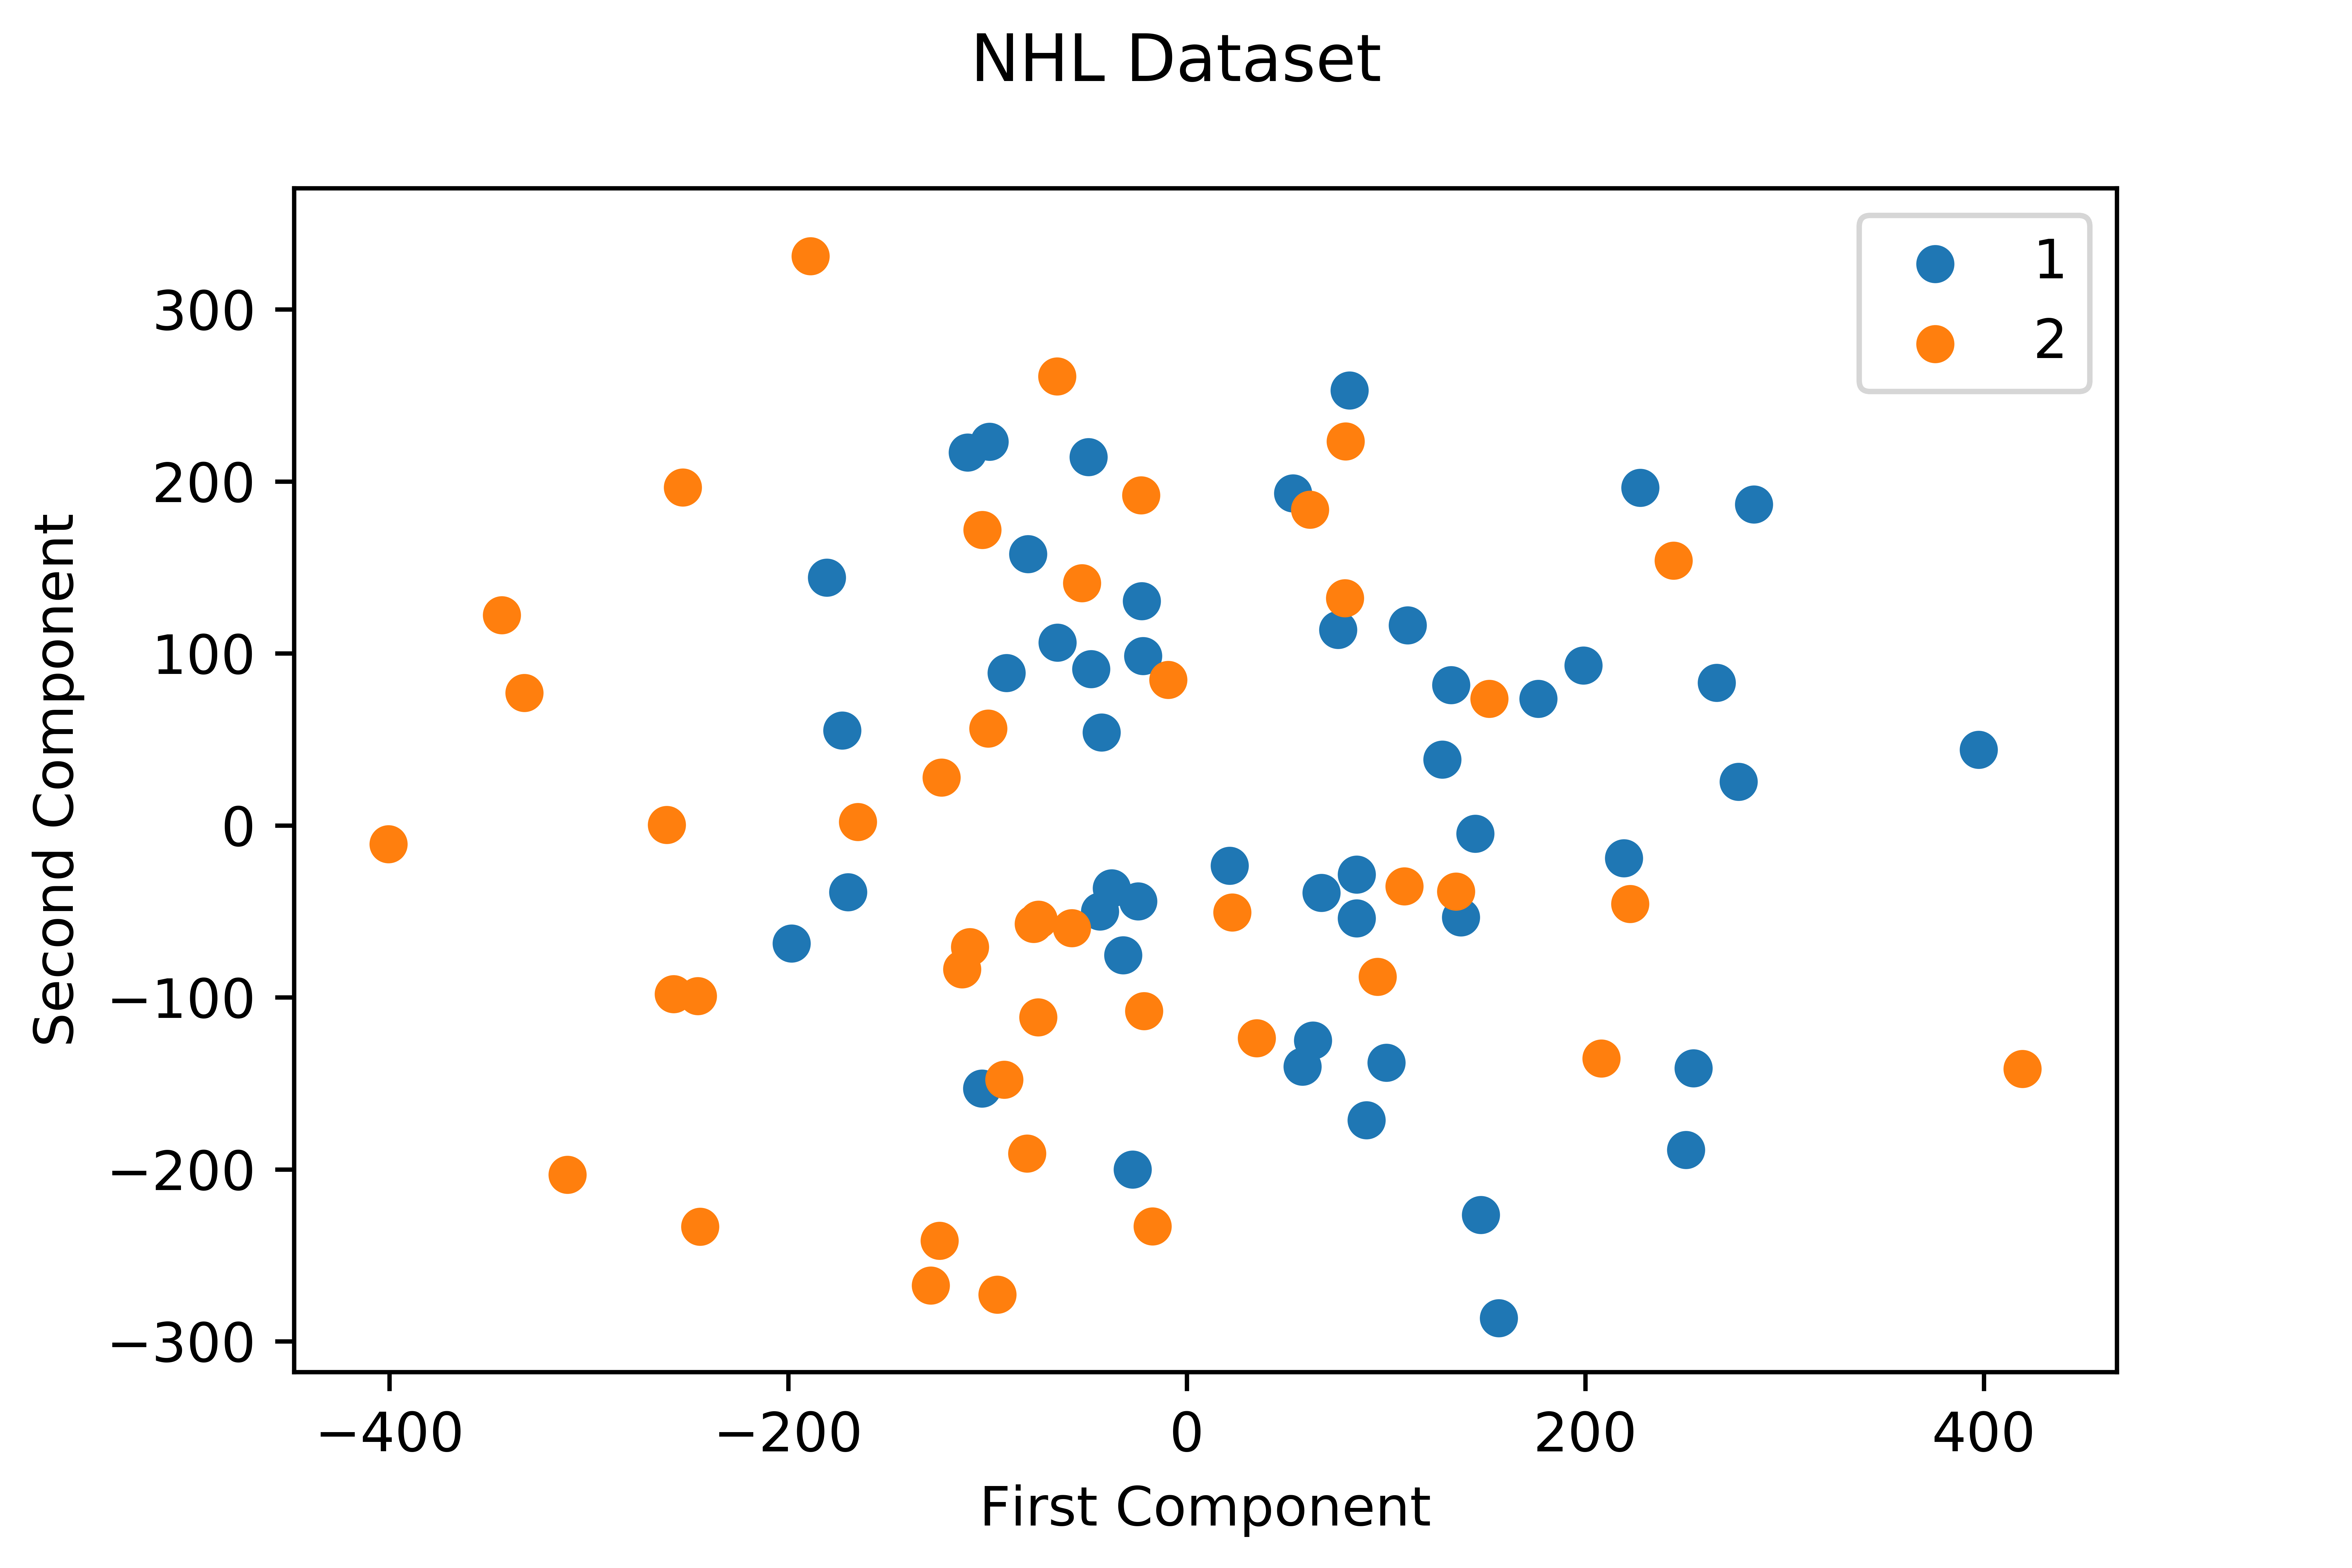
\includegraphics[width=0.8\linewidth]{figures/pca1.png}
          \caption{Sadly, this is pretty useless...}
          \label{fig:pca}
        \end{figure}


      % \subsubsection{Nonnegative Matrix Factorization}
      %   This \emph{might} be useful.
      %   It is currently here mostly as a reminder to think about it.
      %
      % \subsubsection{Randomized Dimensionality Reduction}
      %   Yeah just read what's under the nonnegative matrix factorization section right now...


    % \subsection{Causality??}
    %   \subsubsection{Causal Diagrams}
    %     This actually might be a very useful thing to introduce near the beginning, or just use them throughout (causal and just regular DGMs) to help explain the processes attempting to be modeled.
    %     Particularly in the HMM and Mixture Model sections (obviously)...


    \subsection{Time-Series Forecasting}

      \subsubsection{ARIMA Modeling}

        \paragraph{Team Level}

          \begin{itemize}
            \item[(i)] General performance - wins, goals for, etc.

            \item[(ii)] Specific team performance metrics - PPP, PK, PIM, etc. - to use in classification models for game outcomes \emph{as if} the game already happened (does this make sense?)

          \end{itemize}

        \paragraph{Individual Level (and line level??)}\hfill

          Not particularly different from the team level, just for individuals.
          Obviously, this will encompass different statistics, and therefore different analysis.
          Also, there is quite a bit more that \emph{could} be done here compared with the team level, I just can't really remember what at the moment.


    \subsection{State Estimation}

        \subsubsection{Overview of Various States}
          This is where we explain what we mean by ``state'' in the context of hockey.
          This includes fully observable states, quasi-observable states (quasi-latent??), and latent states.\\

          One example would be team build or style of play.
          Some teams are built to be quick on their feet while others are designed to play physically, with the goal of wearing out the other team.
          We would consider this a quasi-observable state, since you either use ML techniques to determine these states entirely autonomously (unsupervised) or semi-autonomously (semi-supervised), or manually label them based on personal familiarity.\footnote{Or by whether or not a team's name sounds fierce. However, since there is a lack of academic research concerning such methods, it is hard to say how effective it would be.}

          \paragraph{Fully Observable States}
            Description of the fully observable states we deal with.

          \paragraph{Latent (Hidden) States}
            Description of the latent (and quasi-latent) states we deal with.


        \subsubsection{Hidden Markov Models}


        \subsubsection{Mixture Models (Does this go here?)}


        \subsubsection{Kalman Filter (Is this useful...?)}


    \subsection{Reinforcement Learning}
      Could we run reinforcement learning on historical data but as if it were a live stream???
      That is, could we train a model that would predict stuff about a game as its unfolding by using the very large amount of historical data available....??????
      That would be awesome.


  \section{Analysis}


  \section{Conclusion}

  % Appendix
  \pagebreak
  \renewcommand{\thesection}{\Alph{section}}
  \renewcommand{\thesubsection}{\Alph{section}.\arabic{subsection}}
  \renewcommand{\thesubsubsection}{\Alph{section}.\arabic{subsection}.\arabic{subsubsection}}
  \setcounter{section}{0}



  \section{Appendix}
    \begin{figure}[!htb]
      \label{fig:xkcd-ml}
    \centering
      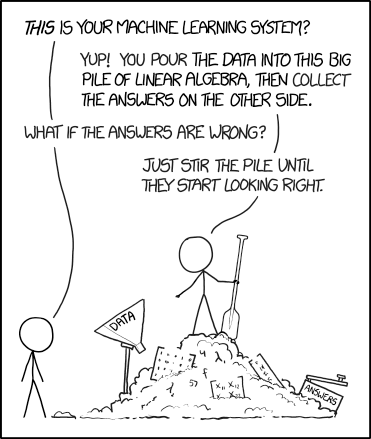
\includegraphics[width=0.6\linewidth]{figures/xkcd-ml.png}
    \caption{For the less technical readers, this is all you really need to know about machine learning and artificial intelligence. (Source: https://xkcd.com/1838/)}
    \end{figure}


\end{document}
